\documentclass[12pt]{article}
\usepackage{amsmath}
\usepackage{amssymb}
\usepackage{derivative}
\usepackage{tikz}

\begin{document}

\title{Backpropagation through recurrent layer}
\author{Kadulin V.}
%\date{}
\maketitle

Let $X \in \mathbb{R}^{N \times T \times D}$ be $D$-dimentional representations of $N$ sequences of length $T$ each, $h \in \mathbb{R}^{N \times H}$ is hidden state of a recurrent cell. Let $g: (x_t, h_t) \rightarrow h_{t+1}$ is a recurrent cell operator, where $x_t \in \mathbb{R}^{N \times D}$ is a batch of $t$-th elements of each sequence, $h_t \in \mathbb{R}^{N \times H}$ is a batch of hidden states at step $t$. $g_t = \tanh(x_t W_x + h_{t-1} W_h + b$). Applying this operator consequentially to each of $T$ slices along second axis of $X$, we will store outputs in $Y \in \mathbb{R}^{N \times T \times H}$. Let $f$ is a scalar function of $Y$. We know $\pdv{f}{Y}$. Derive $\pdv{f}{W_x}$, $\pdv{f}{W_h}$, $\pdv{f}{b}$, $\pdv{f}{X}$, $\pdv{f}{h_0}$.

First, let's derive a single backward step through $g$. Let $x, y, h$ are input, output and hidden state at step $t$ respectively, $h_{t-1}$ -- hidden state at step $t-1$. Let $z$ be the expression inside $\tanh$ function.

$\pdv{f}{z} = \pdv{f}{g} \pdv{g}{z}$

$\pdv{g}{z} = \left( \frac{e^{z} - e^{-z}}{2} \right)^{-2}$

$\pdv{f}{x_t} = \pdv{f}{z} W_x^\top$

$\pdv{f}{W_x} = x^\top \pdv{f}{z}$

$\pdv{f}{h_{t-1}} = \pdv{f}{z} W_h^\top$

$\pdv{f}{W_h} = h_{t-1}^\top \pdv{f}{z}$

$\pdv{f}{b} = \sum_{i=1}^{N} \pdv{f}{z}_i$

Let's consider case $N = 1, T = 2$. So, let $x_t \in \mathbb{R}^D$ be a word representation at step $t$, $h_t \in \mathbb{R}^H$ be a hidden state at step $t$. The computation graph is as follows:

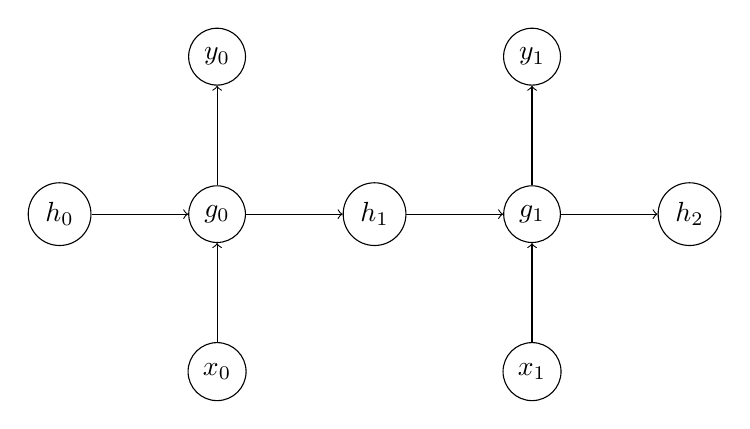
\begin{tikzpicture}[node distance={20mm}, main/.style = {draw, circle}]
\node[main] (1) {$h_0$};
\node[main] (2) [right of=1] {$g_0$};
\node[main] (3) [below of=2] {$x_0$};
\node[main] (4) [above of=2] {$y_0$};
\node[main] (5) [right of=2] {$h_1$};
\node[main] (6) [right of=5] {$g_1$};
\node[main] (7) [below of=6] {$x_1$};
\node[main] (8) [above of=6] {$y_1$};
\node[main] (9) [right of=6] {$h_2$};
\draw[->] (1) -- (2);
\draw[->] (3) -- (2);
\draw[->] (2) -- (4);
\draw[->] (2) -- (5);
\draw[->] (5) -- (6);
\draw[->] (7) -- (6);
\draw[->] (6) -- (8);
\draw[->] (6) -- (9);
\end{tikzpicture}

\begin{itemize}

\item $y_t = h_{t+1}$, different letters here are set to distinguish different cases.
\item $\pdv{f}{g_t} = \pdv{f}{y_t} + \pdv{f}{h_{t+1}}$, where the first term is an upstream derivative, and the second term -- local recurrent layer derivative, passed back between steps.

\end{itemize}

$\pdv{f}{W_x} = \sum_{t=1}^{T} \pdv{f}{W_x}_t$

$\pdv{f}{W_h} = \sum_{t=1}^{T} \pdv{f}{W_h}_t$

$\pdv{f}{b} = \sum_{t=1}^{T} \pdv{f}{b}_t$

$\pdv{f}{X}_{\cdot, t, \cdot} = \pdv{f}{x_t}$

$\pdv{f}{h_0} = \pdv{f}{z_1} W_h^\top$

\end{document}